% TALK ABOUT HYDRA AND HOW THE ORGANISMS CAN REGENERATE PARTS OF ITS BODY.

\section{Hydra Morphogenesis and regenerative properties}

\subsection{Anatomy of a Hydra}

Hydras (\textit{diploblastic metazoan hydra}) are fascinating creatures. Small freshwater polyps, Despite their rather small size of roughly 5mm of length in average, they are capable of extraordinary regenerative properties that allow them to fully reconstruct their body out of a very small portion of tissue (\ref{hydraregen}).
\begin{figure}[h]
\label{hydraregen}
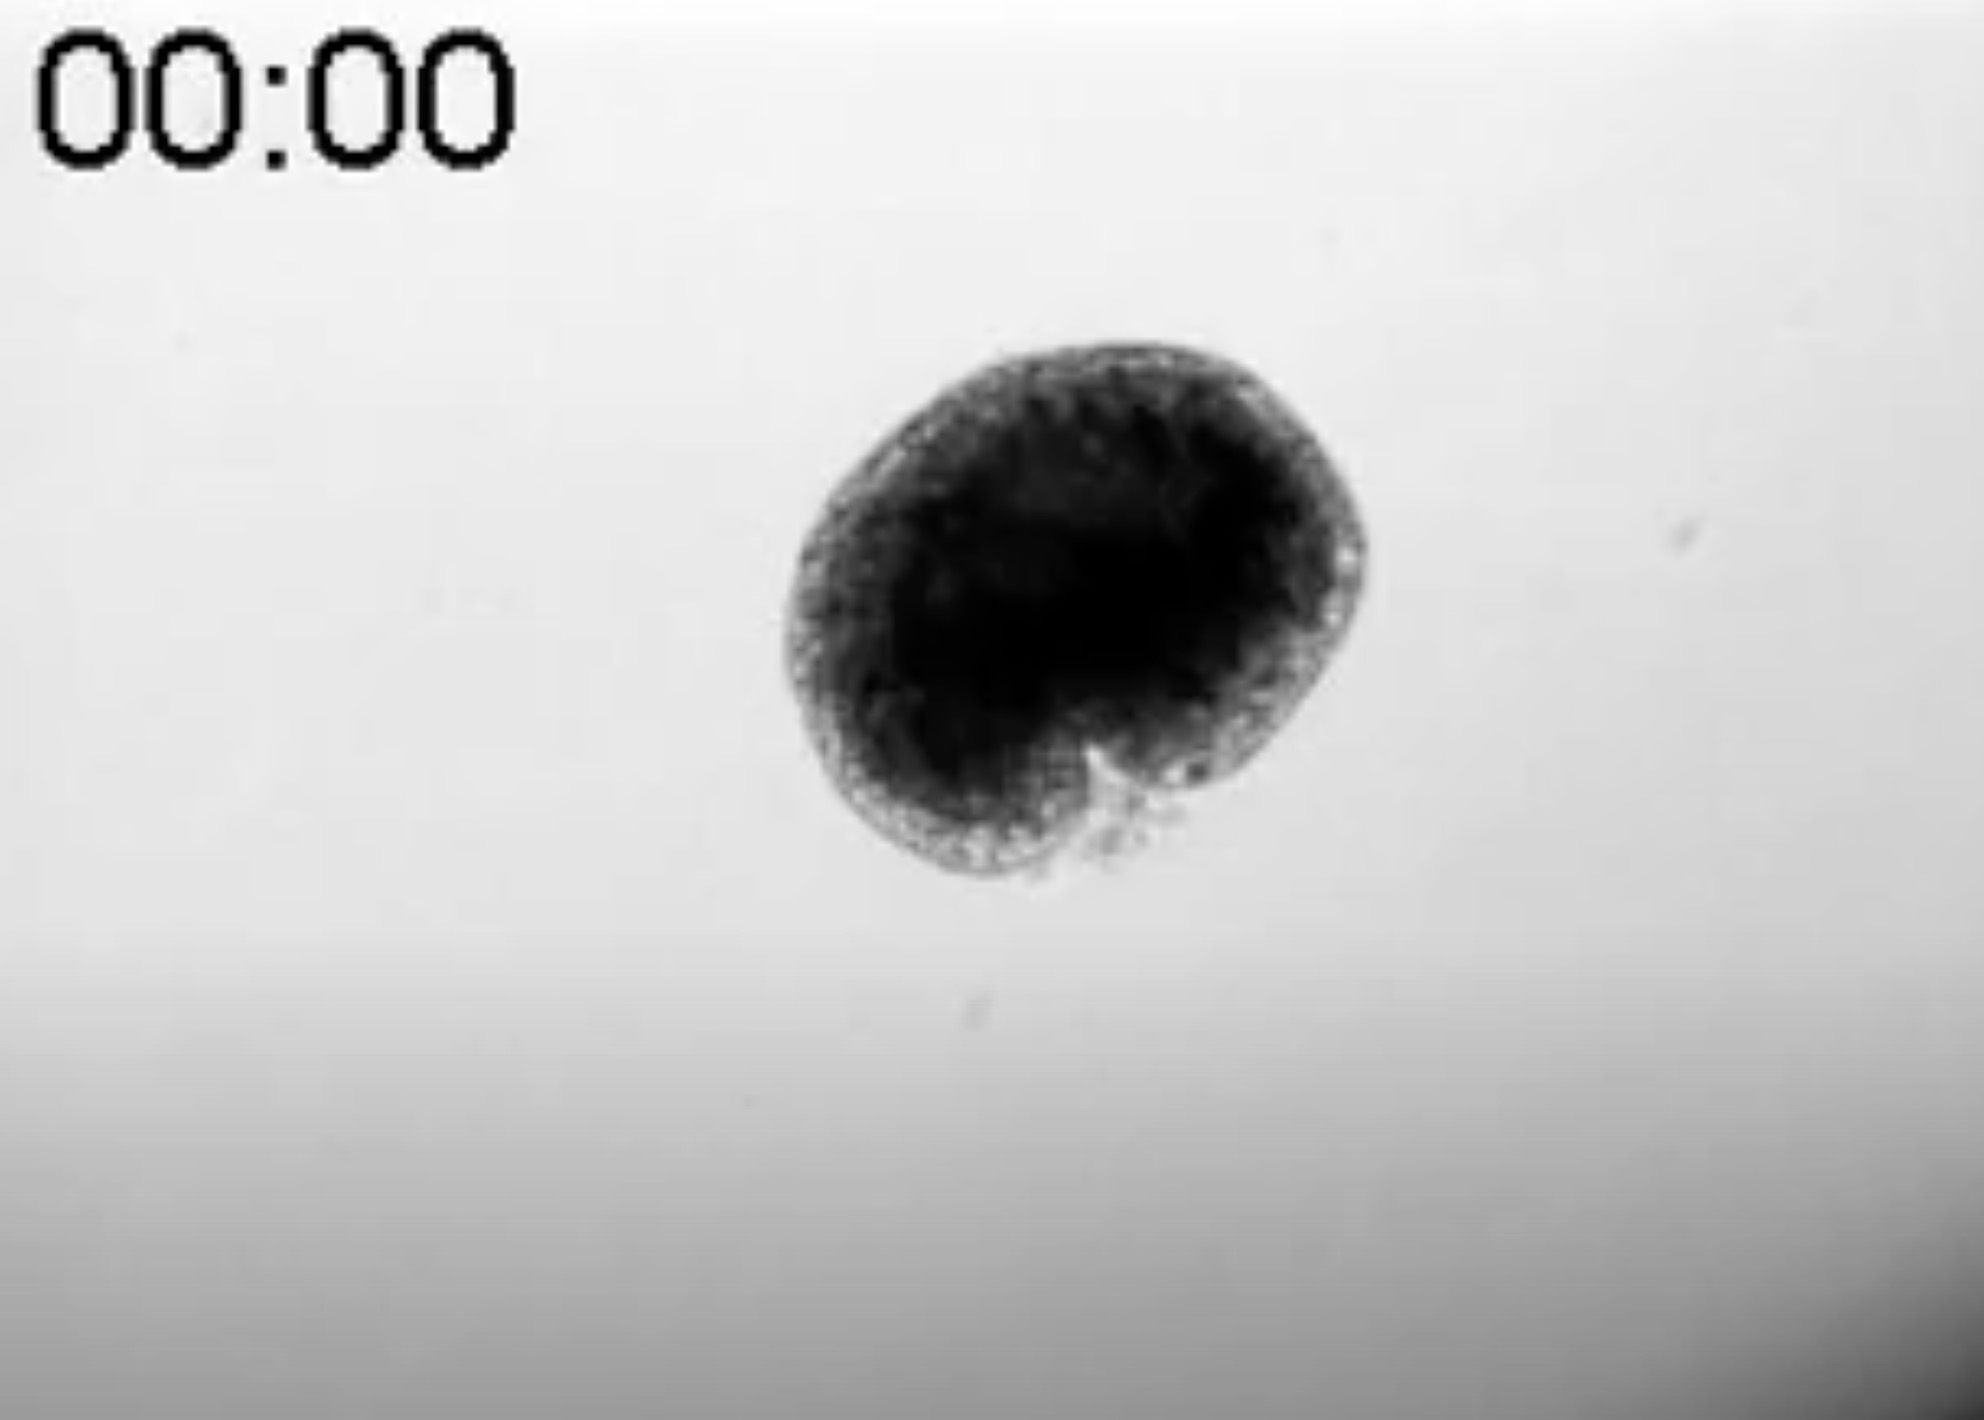
\includegraphics[width=0.19\textwidth]{figures/hydra_growth1}
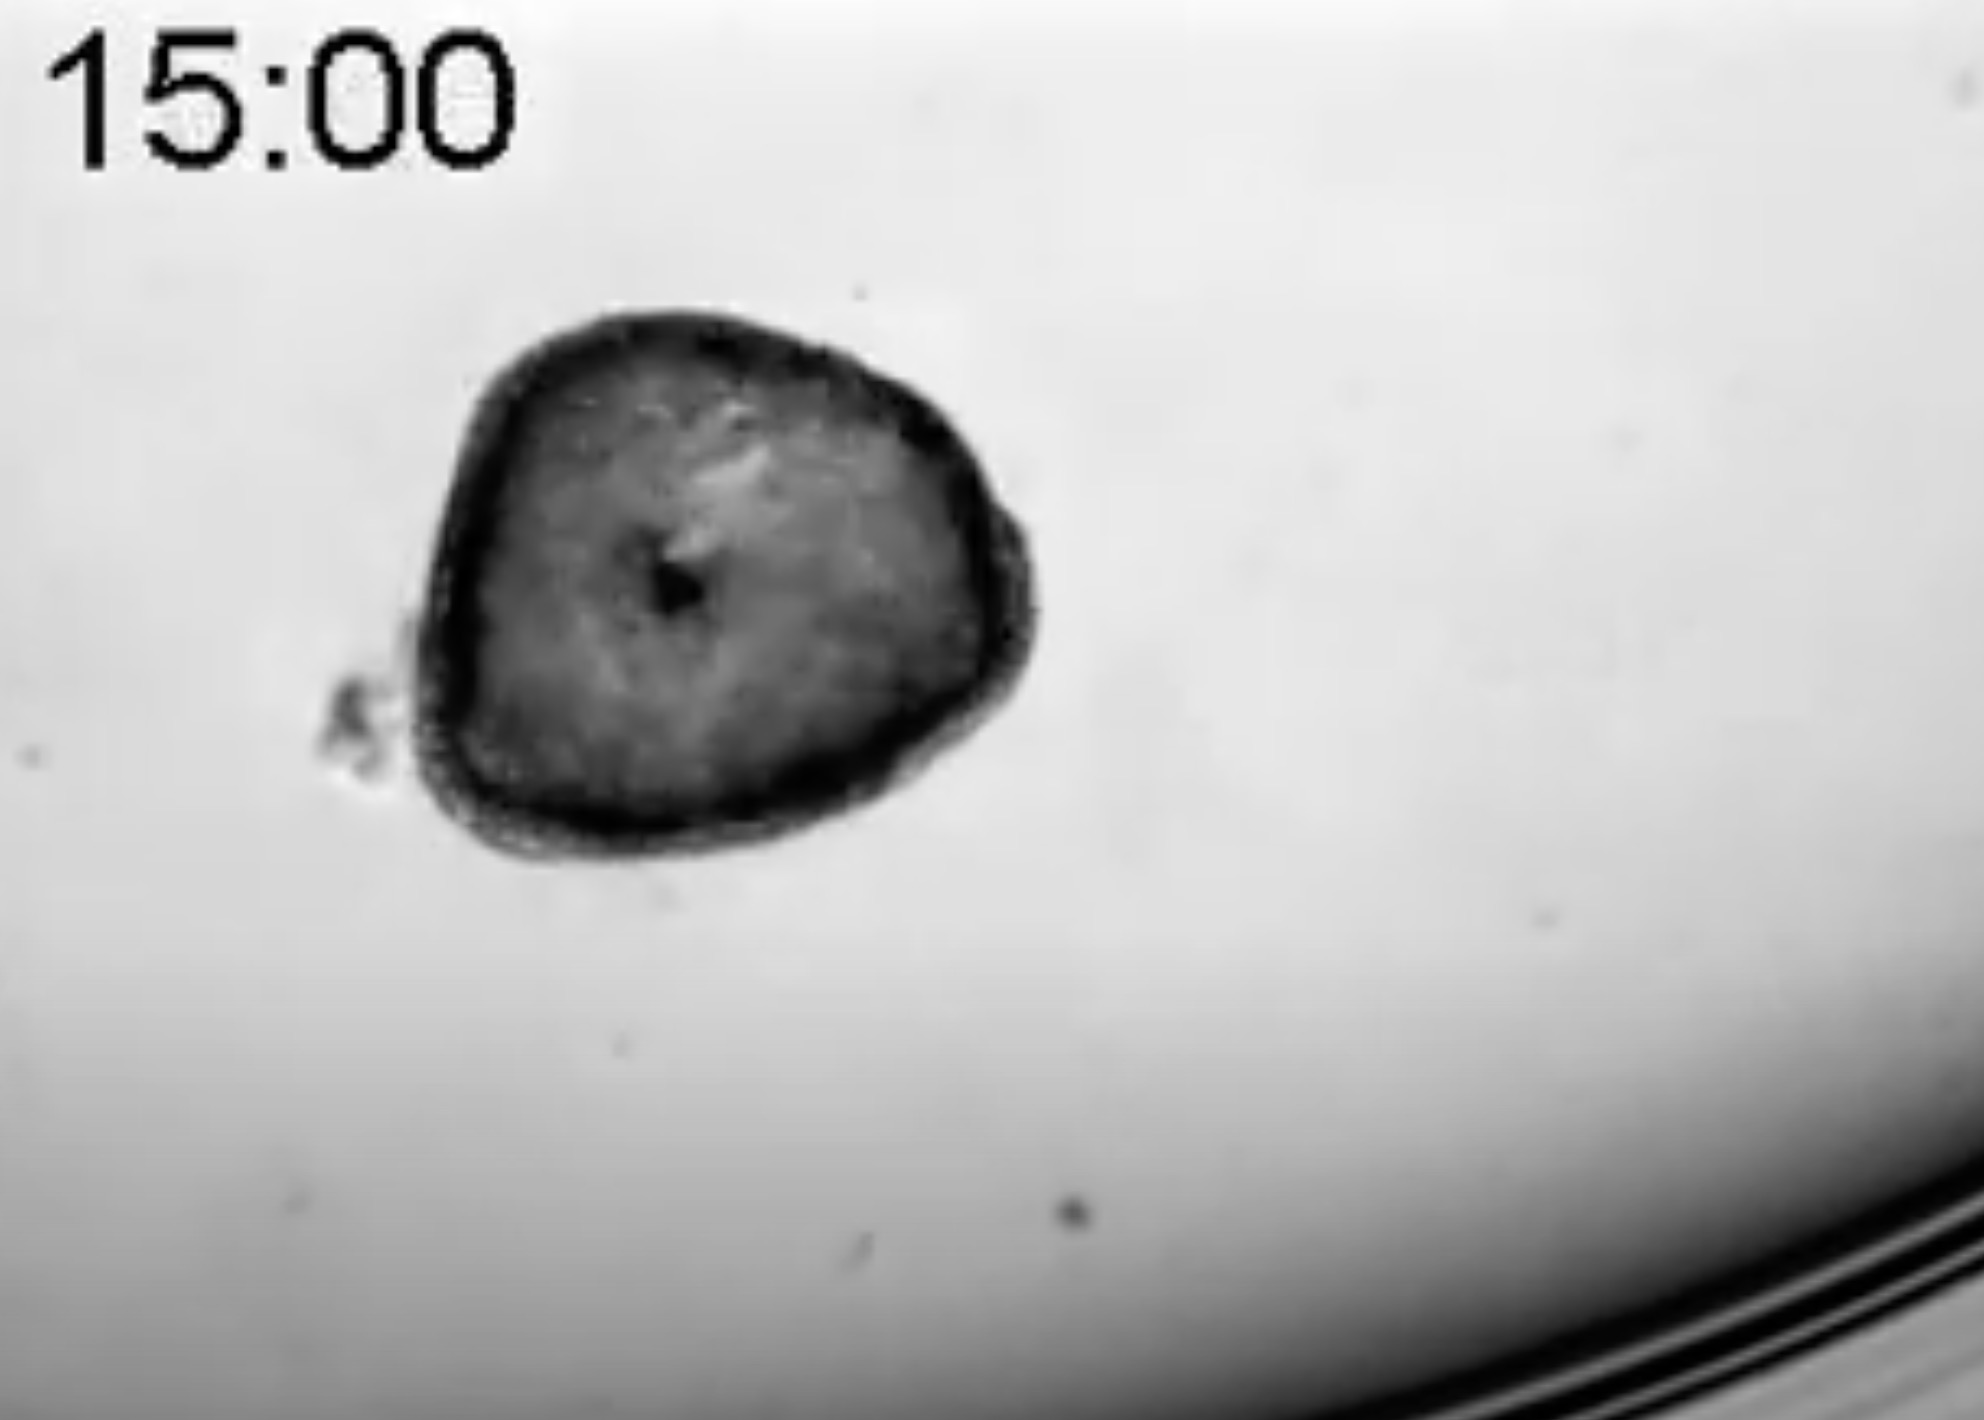
\includegraphics[width=0.19\textwidth]{figures/hydra_growth2}
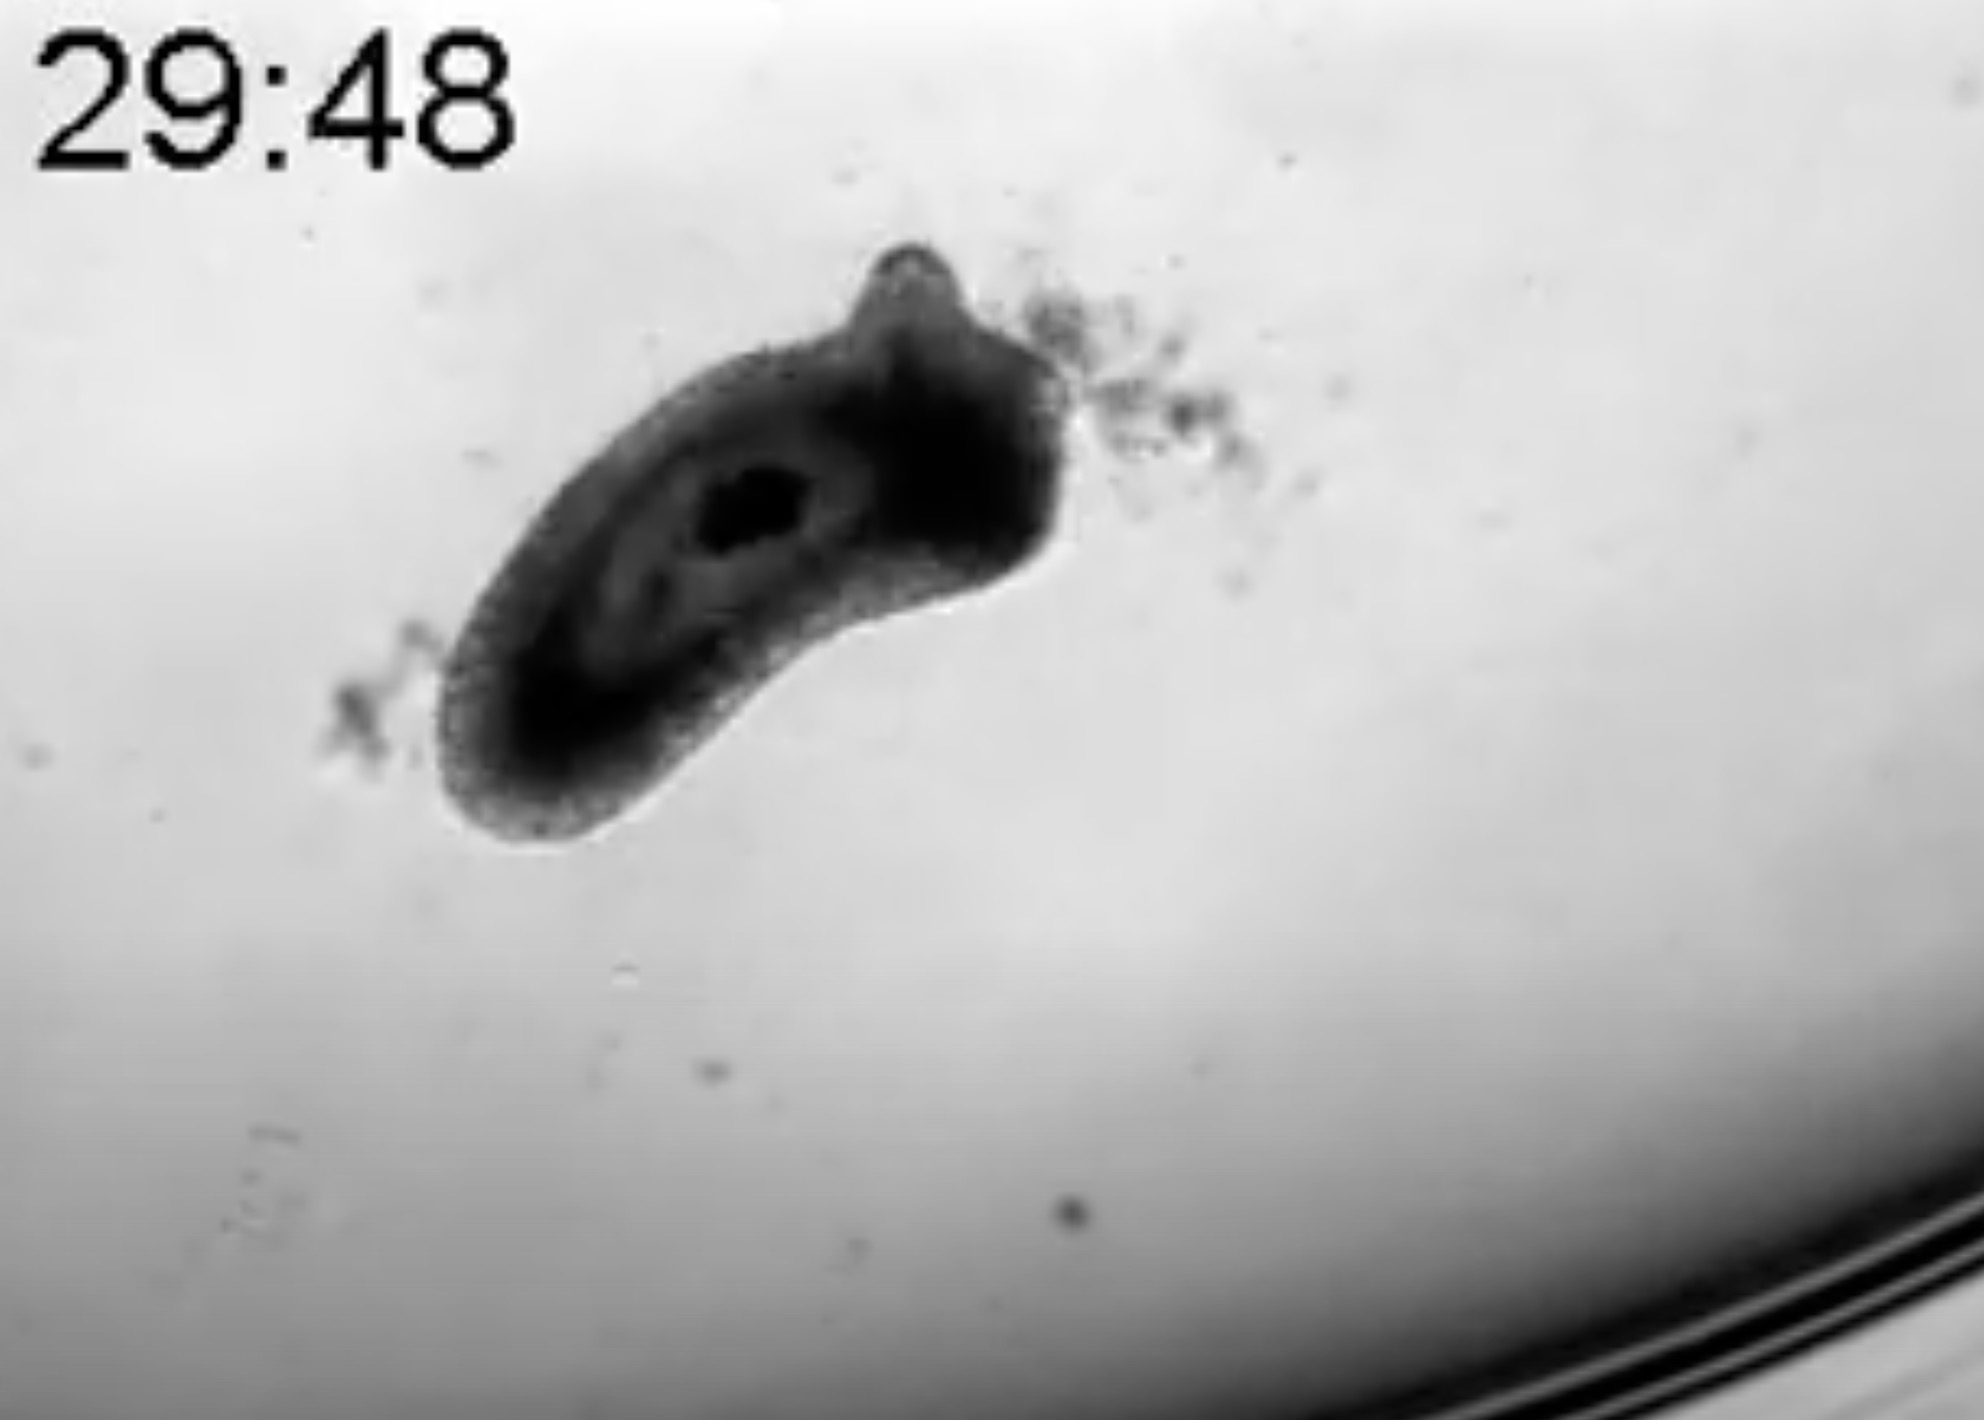
\includegraphics[width=0.19\textwidth]{figures/hydra_growth3}	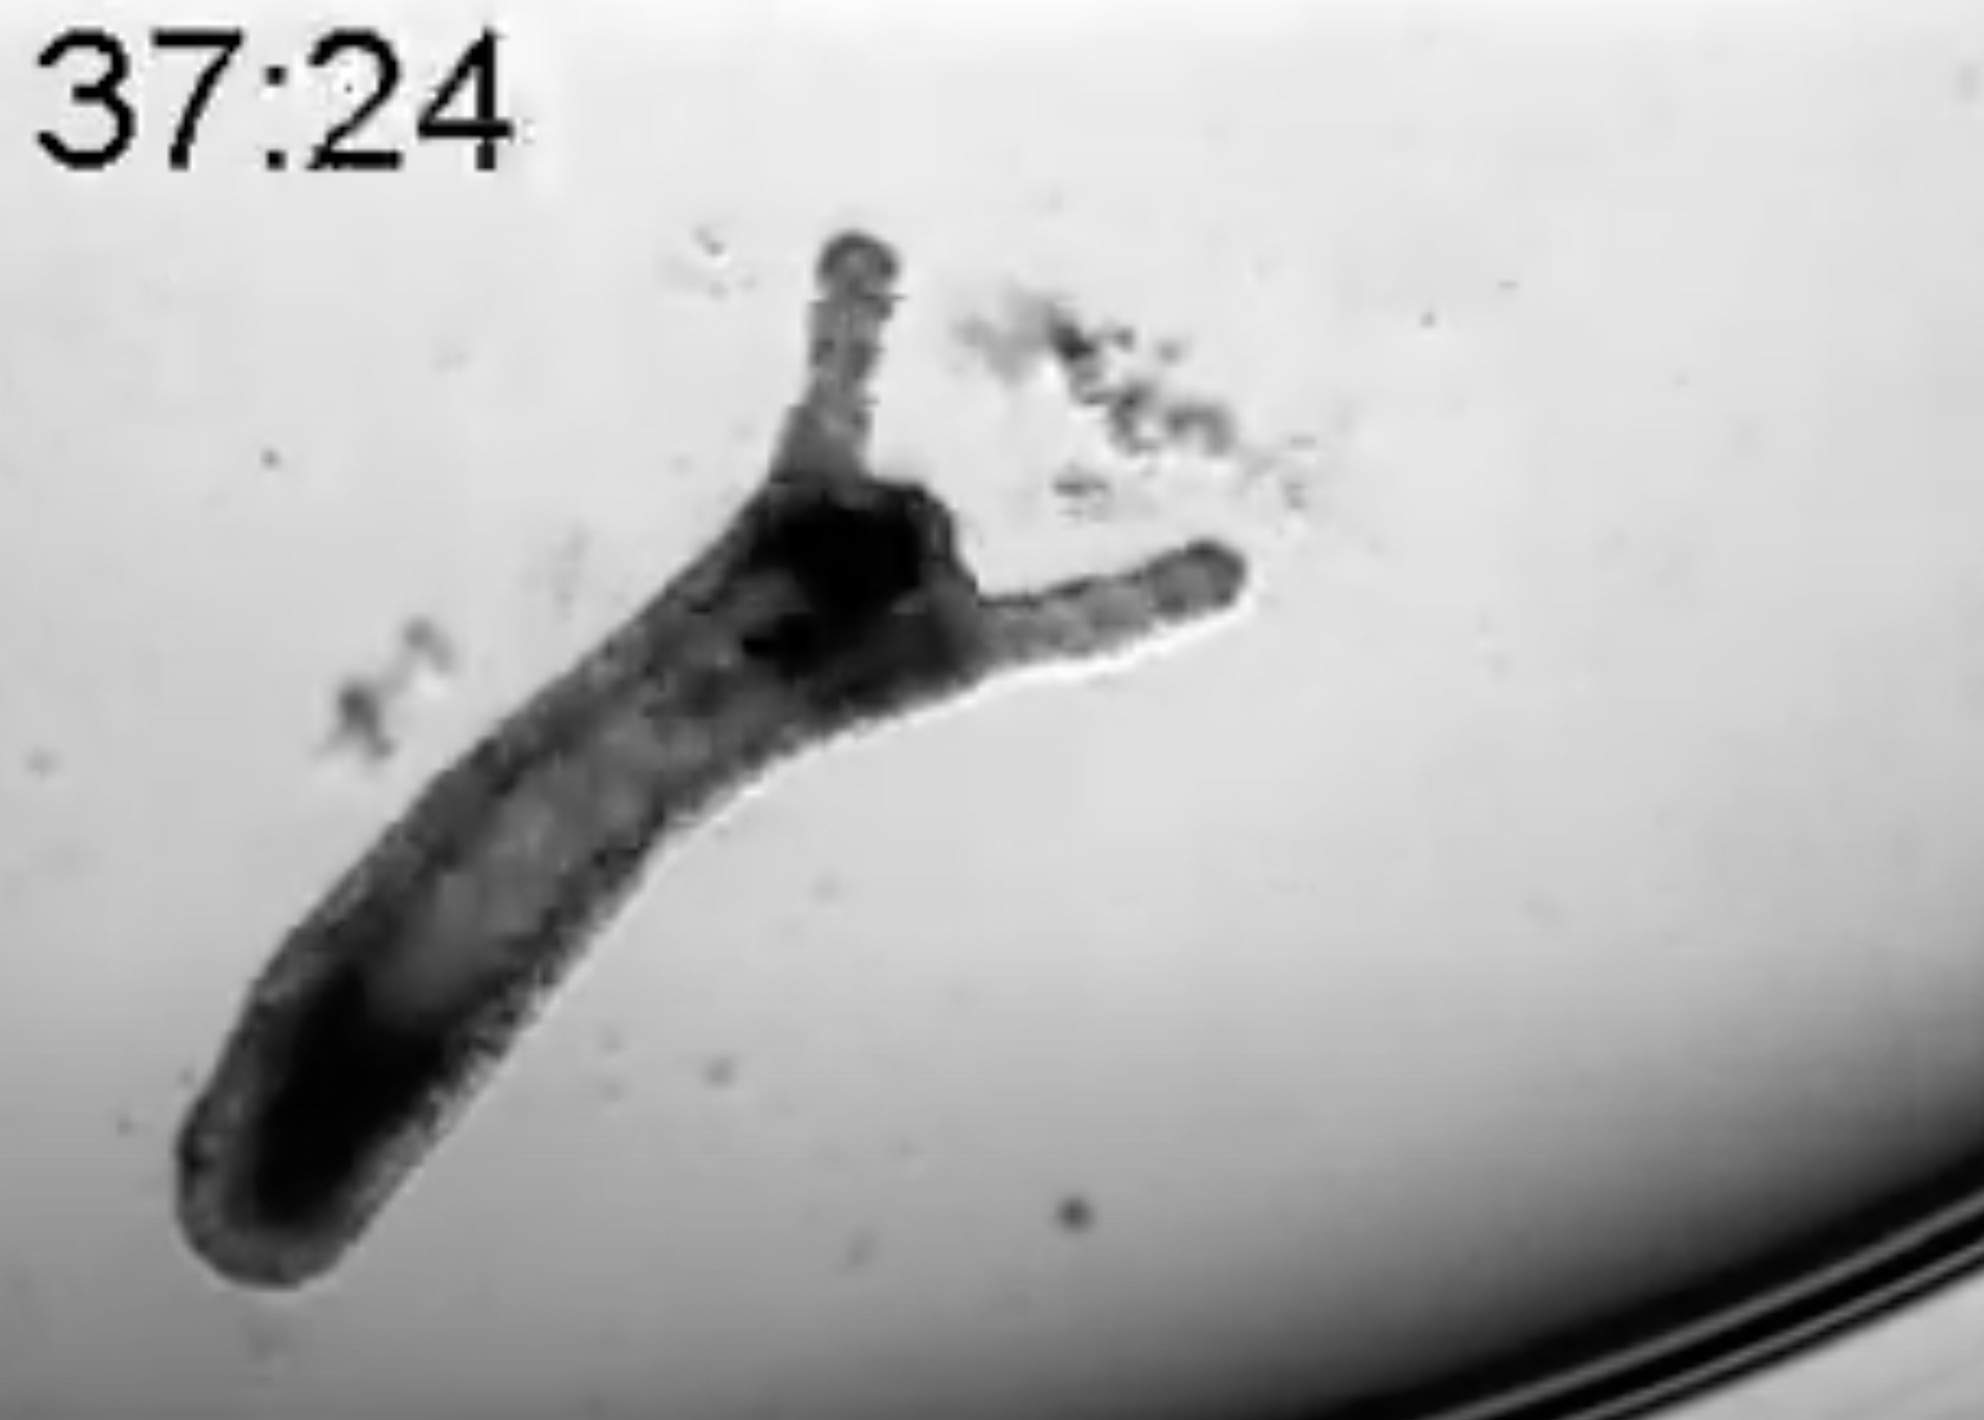
\includegraphics[width=0.19\textwidth]{figures/hydra_growth4}
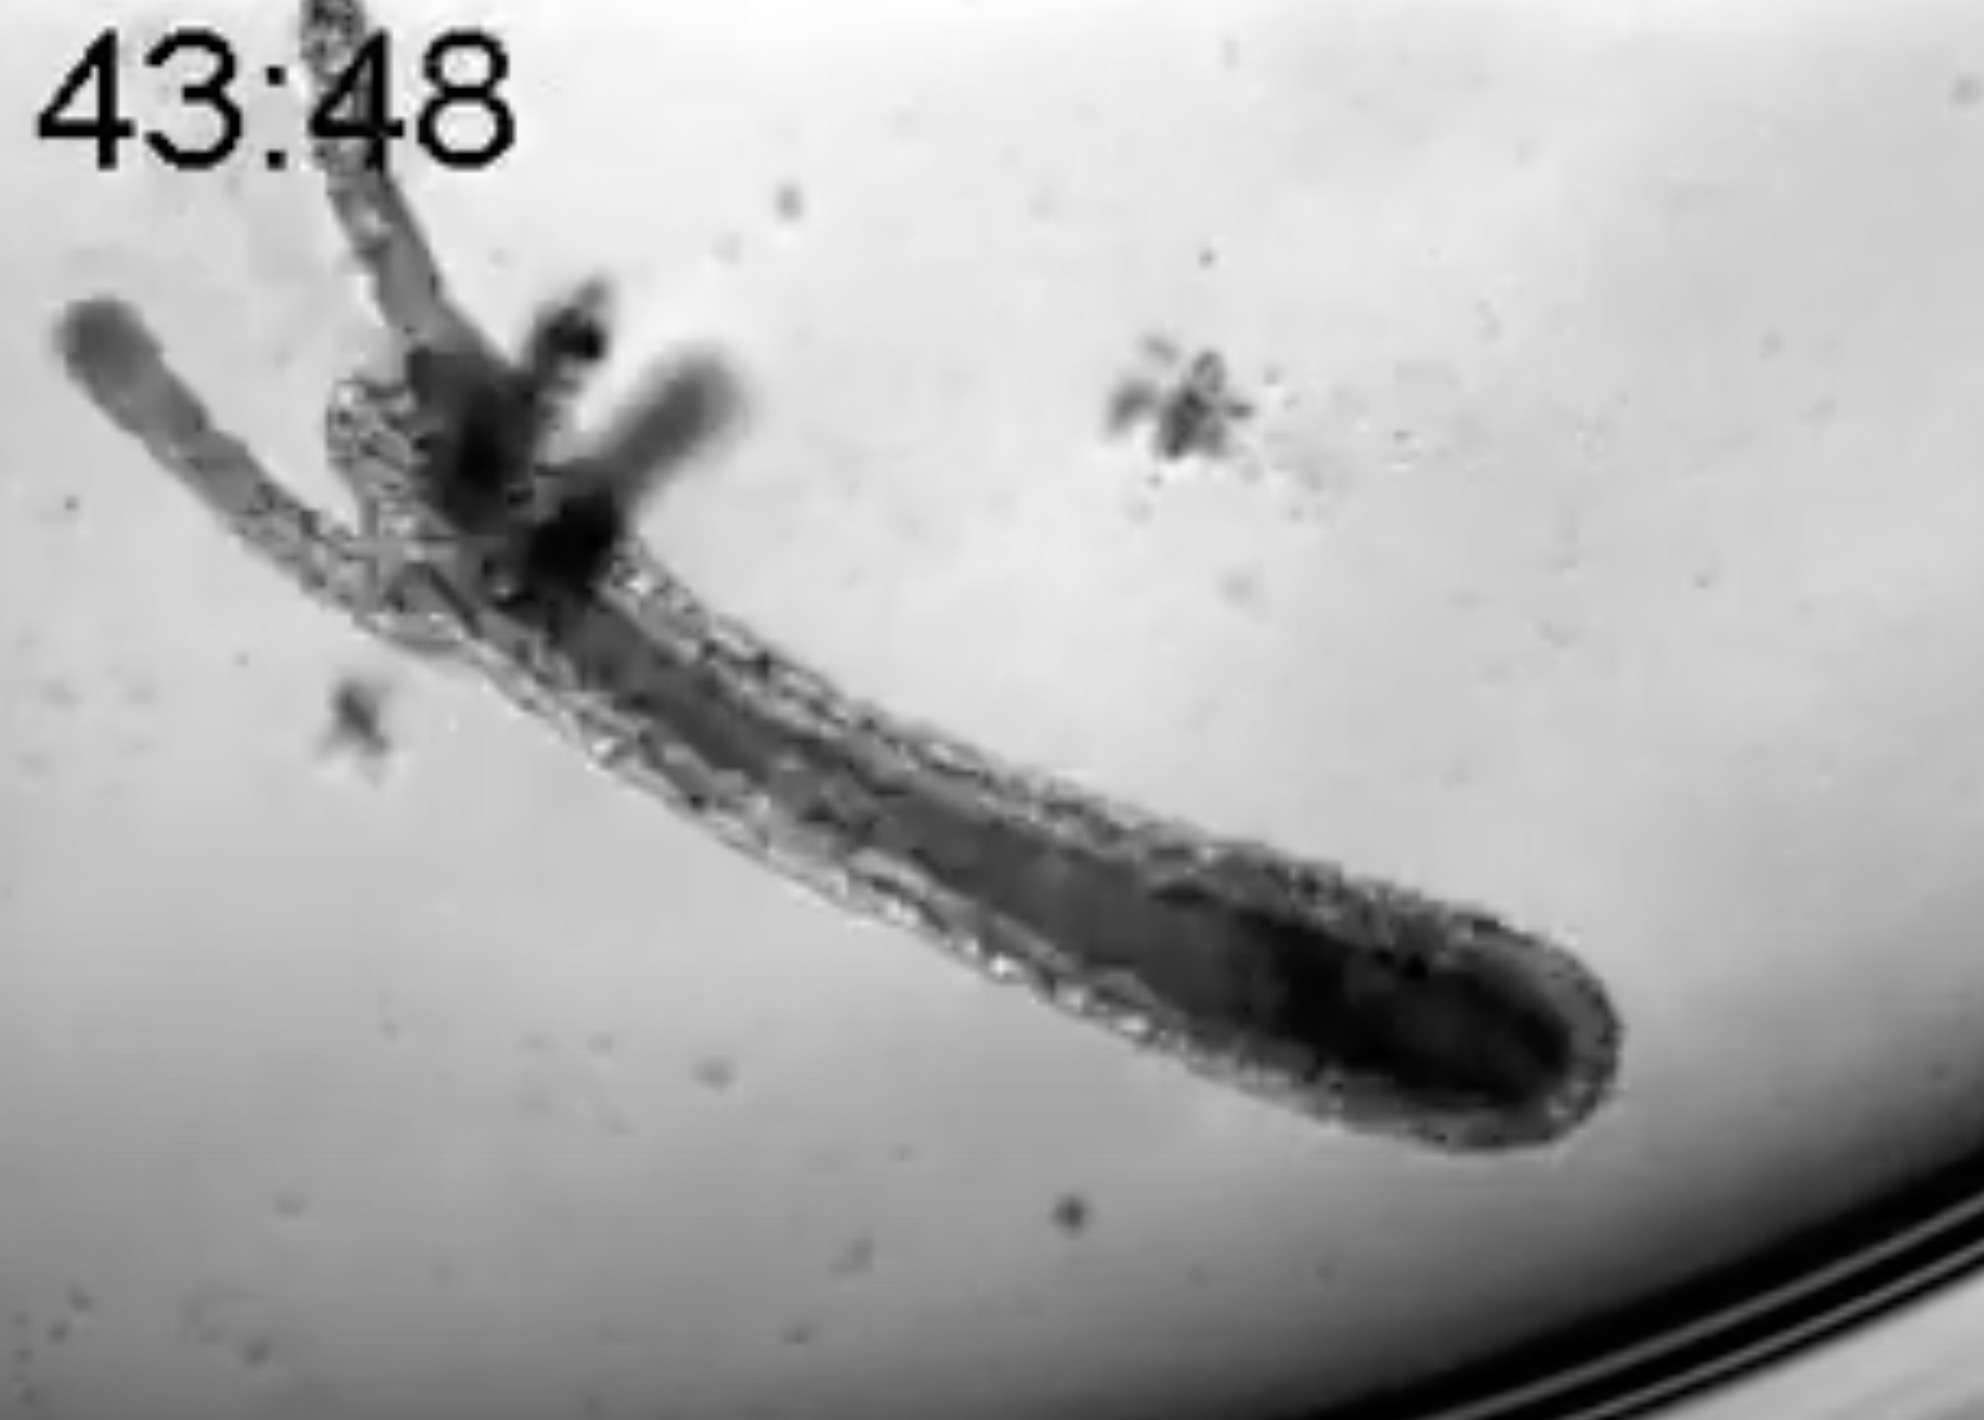
\includegraphics[width=0.19\textwidth]{figures/hydra_growth5}
\caption{Sequence of pictures taken under a traditional microscope. It shows how hydras are capable of regenerating their entire body using small extracted samples of tissue coming from the body column of another hydra (tissue diameter is about 100 $\mu$m). The timestamp on each picture is formatted as "hours:minutes", meaning the entire regeneration process takes less than two days to occur.}
\end{figure}

Their body is composed of essentially three regions: the head, body column and foot. Spatially speaking, the small cnidarian is symmetrically organized around the oral-aboral axis giving it its hollow, tubular shape. Taking a closer look on each part, one can notice that the head is composed of two sub-regions. One being a set of tentacles while the other one is called hypostome and acts as a mouth (it is also the only orifice in the whole organism). The foot, on the other hand is composed of a basal disc that allows hydras to stick to underwater leaves and rocks - among others -. Lastly, the body column is a long hollow tube made of cells undergoing constant mitosis through the life of the polyp, this process ensures a constant cellular turnover of the derm.

\begin{remark}[Hydra reproduction]
	The way hydras reproduce is very peculiar but is of great interest to the scientific community since they are able to give birth either sexually or through natural cloning, see figure \ref{fig:hydrareprod} (the latter being the most common way of reproduction in labs). The main difference between these two methods is that asexual reproduction preserves the totality of information in one individual, letting one the ability to duplicate a specific hydra with nice genetic information if they wish. This considerably enhances the pace at which experiments occur while reducing the randomness factor due to genetics (therefore improving reproducibility of experiments). 
\end{remark}

%\begin{figure}[h!]
%	\label{hydrareprod}
%	\centering
%	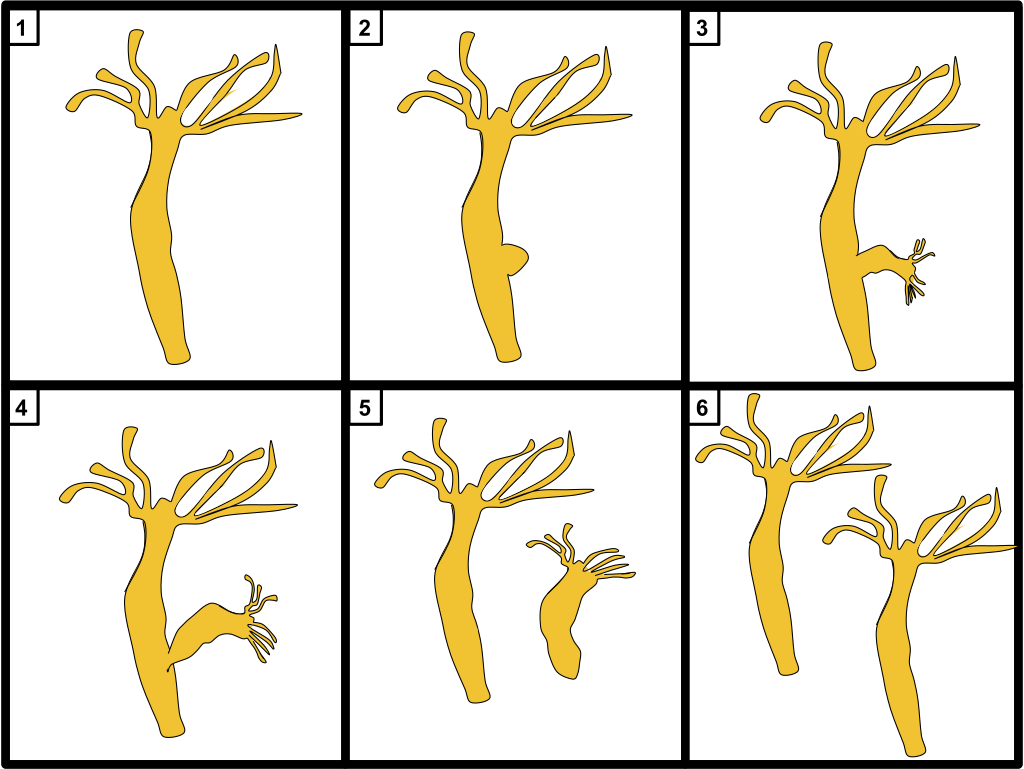
\includegraphics[width=0.6\textwidth]{figures/hydra_asexual.png}
%	\caption{Illustrated process of asexual reproduction in Hydra. A new head grows on the body column at the top of the peduncle (this small lump is familiarly call "the bud") and keeps growing until it detaches from the "adult"'s body. Once detached, the new individual sticks to nearby rocks or leaves and keeps growing until adult size is reached. (credit: picture from \cite{Neupane2022})}
%\end{figure}

\begin{figure}[h]
	\floatbox[{\capbeside\thisfloatsetup{capbesideposition={right,center},capbesidewidth=0.6\linewidth}}]{figure}[\FBwidth]
	{\caption{Illustrated process of asexual reproduction (natural cloning) in Hydra. A new head grows on the body column at the top of the peduncle (this small lump is familiarly call "the bud") and keeps growing until it detaches from the "adult"'s body. Once detached, the new individual sticks to nearby rocks or leaves and keeps growing until adult size is reached. (credit: picture from \cite{Neupane2022})}\label{fig:hydrareprod}}
	{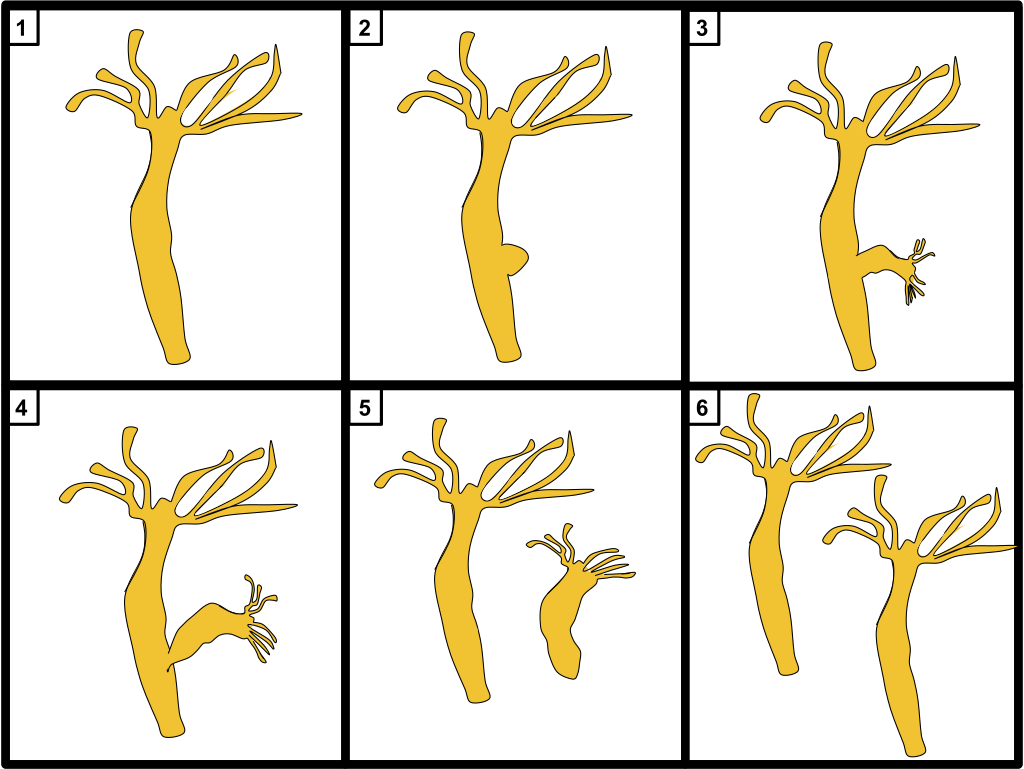
\includegraphics[width=0.9\linewidth]{figures/hydra_asexual.png}}
\end{figure}


  

\subsection{A few words about Wnt proteins}


\subsection{Position-based regrowth and grafting experiments}